	\documentclass[10pt,oneside]{CBFT_book}
	% Algunos paquetes
	\usepackage{amssymb}
	\usepackage{amsmath}
	\usepackage{graphicx}
	\usepackage{libertine}
	\usepackage[bold-style=TeX]{unicode-math}
	\usepackage{lipsum}

	\usepackage{natbib}
	\setcitestyle{square}

	\usepackage{polyglossia}
	\setdefaultlanguage{spanish}
	



	\usepackage{CBFT.estilo} % Cargo la hoja de estilo

	% Tipografías
	% \setromanfont[Mapping=tex-text]{Linux Libertine O}
	% \setsansfont[Mapping=tex-text]{DejaVu Sans}
	% \setmonofont[Mapping=tex-text]{DejaVu Sans Mono}

	%===================================================================
	%	DOCUMENTO PROPIAMENTE DICHO
	%===================================================================

\begin{document}


% =================================================================================================
\chapter{Simetrías en mecánica cuántica}
% =================================================================================================

En mecánica clásica tenemos el teorema de Noether 
\[
	\partial p_i = cte.
\]
Y $\mathcal{H}, \mathcal{L}$ no cambian con la transformación $q_i \longrightarrow q_i + \delta q_i$
\[
	\partial 
\]

En mecánica cuántica definiremos un operador unitario $\$$ asociado a traslación/rotación. Pensemos en una 
transformación infinitesimal dada por $\$$
\[
	\$
\]

Sea el H invariante frente a $\$$, entonces 
\[
	SHS =
\]

Esto significa que el autovalor no varía con el tiempo, Como $[H,G]=0$ se tiene 
\[
	no dege 
\]

\subsection{Simetría de paridad}

Transforma un RHS en LHS. Es decir que hace 
\[
	\vb{x} \longrightarrow - \vb{x}
\]
y solicitaremos un operador unitario llamado paridad que verifique 
\[
	\Ket{\alpha} \longrightarrow \Pi\Ket{\alpha} = \Ket{\alpha'}
\]
si $\Pi$ es unitario y $\Pi^1=\mathbb{1}$ entonces es hermítico.
\begin{figure}[htb]
	\begin{center}
	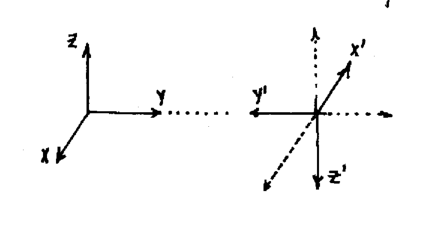
\includegraphics[width=0.6\textwidth]{images/teo2_16.pdf}
	\end{center}
	\caption{}
\end{figure} 
Queremos que refleje el $\Braket{\hat{x}}$ 
\[
	a
\]
anticonmuta con \vb{x}.
Debido a ello 
\[
	a
\]
como $\hat{\Pi}$ no depende del tiempo 
\[
	d
\]
y vemos que anticonmuta con \vb{p}.
\vb{x}, \vb{p} son operadores impares. En cambio $\vb{L}=\vb{x}\times\vb{p}$ es un operador par, entonces 
\[
	[] = 0
\]
\begin{figure}[htb]
	\begin{center}
	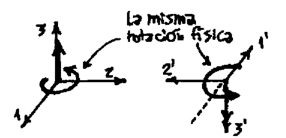
\includegraphics[width=0.6\textwidth]{images/teo2_17.pdf}
	\end{center}
	\caption{}
\end{figure} 
Que conmuta con \vb{J} puede verse de pedirle que 
\[
	[] = 0 \longrightarrow [] = 0 ,
\]
cosa que vale en mecánica clásica, entonces 
\[
	R
\]
\[
	\Box
\]
\[
	\Box
\]

\subsection{Función de onda bajo paridad}

\[
	\Psi
\]
y entonces la función de onda de un estado al que se le aplicó paridad será 
\[
	\Psi
\]

Sea $\Ket{\alpha}$ autoestado de paridad, entonces 
\[
	a
\]
los autovalores serán $\pm 1$
\[
	=
\]
no toda función de onda tiene paridad bien definida.

\[
	\vb{x}
\]
\[
	=
\]
\[
	\Pi
\]
Como $[\vb{L},\hat{\Pi}]=0$ un autoestado de \vb{L} es autoestado de $\hat{\Pi}$ .

\subsection{Teorema}

Sea 
\[
	autoestado 
\]

La demostración 
\[
	()
\]
\[
	2
\]
\[
	3
\]

Un caso donde falla el teorema 
\[
	caso
\]
\[
	caso mas
\]

\subsection{Reglas de selección de paridad $\Pi$}

Sean $\Ket{\alpha}, \Ket{\beta}$ autoestados de paridad 
\[
	\Pi
\]
\[
	\Braket{||}
\]

\begin{itemize}
 \item Operadores impares solo conectan estados de paridad opuesta
 \[
	a
 \]
 \item Operadores pares solo conectan estados de la misma paridad 
 \[
	b
 \]
\end{itemize}

\[
	= 0
\]
\[
	c
\]

\section{Inversión temporal (reversión de movimiento)}

En mecánica clásica sería {\it pasar la película hacia atrás}
\[
	t \longrightarrow -t
\]
En sistemas sin fuerzas disipativas se tiene 
\[
	m \ddot{x} =
\]

En mecánica cuántica tendremos 
\[
	i \hbar 
\]
\[
	=
\]
no es solución de Schrödinger. 
Pero notemos que $\Psi^*(x,-t)$ cumple la ecuación de Schrödinger
\[
	i\hbar
\]

Entonces necesitamos un operador que respete esta característica. Necesitaré el producto interno conjugado 
\[
	\Psi
\]
El operador involucrado no será unitario 
\[
	\Ket{\tilde{\alpha}} = 
\]
Si $\hat{\Theta}$ unitario se conserva el producto interno 
\[
	=
\]

Pediremos antiunitariedad y antilinealidad al operador $\hat{\Theta}$
\[
	=
\]
\[
	=
\]

Todo operador antiunitario y antilineal puede escribirse como producto 
\[
	\Theta = U K
\]
donde $U$ es unitario y $K$ la conjugación compleja. $K$ no cambia los autoestados, porque en base canónica 
un autoestado tiene un solo elemento (1) que no es nulo.
\[
	K
\]

Veamos que $UK$ es antiunitario 
\[
	=
\]

\[
	=
\]
\[
	=
\]

Notemos que no se define $\hat{\Theta}^\dagger$ actuando sobre bras. La demostración anterior esperó a 
quitarse de encima $\hat{K}$ para hacer dual conjugado al $\Ket{\tilde{\beta}}$.

\subsection{Operadores ante $\hat{\Theta}$}

Usaremos la notación 
\[
	\Ket{\tilde{\alpha}} = \hat{\Theta} \Ket{\alpha}
\]
donde hay que tener en cuenta 
\[
	= \mathbb{1}
\]

Sería razonable esperar que 
\[
	= -
\]
Sea $\hat{\mathbb{O}}$ un operador hermítico 
\[
	=
\]
Luego metemos un $=1$
\[
	=
\]

Notamos que no se aplica $\Theta$ sobre bra alguno y tenemos $\Theta$ no unitario. Entonces requeriremos 
\[
	=
\]
como para $\vb{p},\vb{J}$ operadores impares 
\[
	=
\]
y $\vb{x}$ operador par.

Los operadores pares conmutan con $\Theta$,
\[
	= =
\]
\begin{figure}[htb]
	\begin{center}
	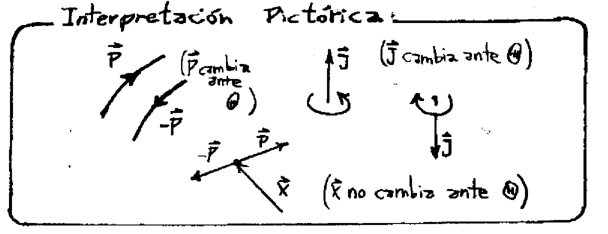
\includegraphics[width=0.6\textwidth]{images/teo2_18.pdf}
	\end{center}
	\caption{}
\end{figure} 
Hamiltoniano ante reversión de movimiento. Veamos la reversión de un sistema en estado $\Ket{\alpha}$
\[
	=
\]
Si el hamiltoniano es invariante ante reversión temporal debería ser lo mismo 
\[
	=
\]
es decir que estamos pidiendo que se obtenga el mismo estado 
\begin{itemize}
 \item Si revertimos el movimiento y evolucionamos $\delta t$.
 \item Si evolucionamos hacia atrás $-\delta t$ y revertimos el movimiento.
\end{itemize}
\begin{figure}[htb]
	\begin{center}
	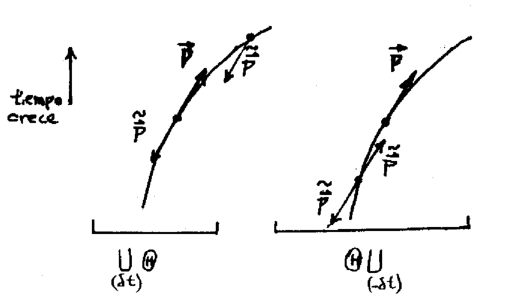
\includegraphics[width=0.6\textwidth]{images/teo2_19.pdf}
	\end{center}
	\caption{}
\end{figure} 
Veamos que vale lo anterior, pensando que si vale se tiene 
\[
	=
\]
\[
	=  \qquad [H,\Theta]=0
\]

Si $\Theta$ era unitario teníamos la relación de anticonmutación $\{ H, \Theta \}=0$ lo cual lleva a absurdos.
\[
	a
\]
Si $\{ H,\Theta \} = 0$
\[
	= \text{H debe ser par frente a $\Theta$}
\]

\subsection{Función de onda}

Sea en $t=0$ un sistema en el estado $\Ket{\alpha}$
\[
	= = 
\]
\[
	\Psi
\]
Esto era lo que {\it vimos} en la ecuación de Schrödinger.

\subsection{Reversión de movimiento sobre \vb{J}}


no tiene sentido porque $J_x,J_y,J_z$ no conmutan entre ellos. Analizaremos $\Ket{\ell,m}$
\[
	\Theta \Ket{\vb{J}} 
\]
\[
	\equiv 
\]

Lo que hace $\Theta$ es invertir la componente de $\hat{z}$ y alterar la fase. Se ve que 
\[
	\Theta^2 = \mathbb{1}
\]

\subsection{Reversión para sistemas de spin $1/2$}

Sea un estado general up de spin $\Ket{\hat{n};+}$, que se obtiene con dos rotaciones 
\[
	Sn
\]
\[
	\Theta
\]
\[
	a
\]
\[
	b
\]
\[
	c
\]

\subsection{Teorema}

Sea $H$ invariante ante $\Theta$ y los $\Ket{n}$ no degenerados, entonces la autofunción de energía puede 
hacerse real tomando una fase apropiada.

Demostración 
\[
	H \Theta  \Ket{n} =
\]
\[
	=
\]
\[
	=
\]

Si le aplico al sistema transformaciones dadas por operadores que conmutan con el H no lo sacamos del 
autoestado en que se encuentra con el paso del tiempo.
En ese sistema solo será razonable medir variables representadas por esos operadores; puesto que de lo 
contrario estamos alterando el sistema y nos es imposible saber donde ha quedado.



% \bibliographystyle{CBFT-apa-good}	% (uses file "apa-good.bst")
% \bibliography{CBFT.Referencias} % La base de datos bibliográfica

\end{document}
